\newpage
\section{Durchführung}
    \subsection{Versuchsaufbau}

        \FloatBarrier

        \begin{figure}[h]
          \centering
          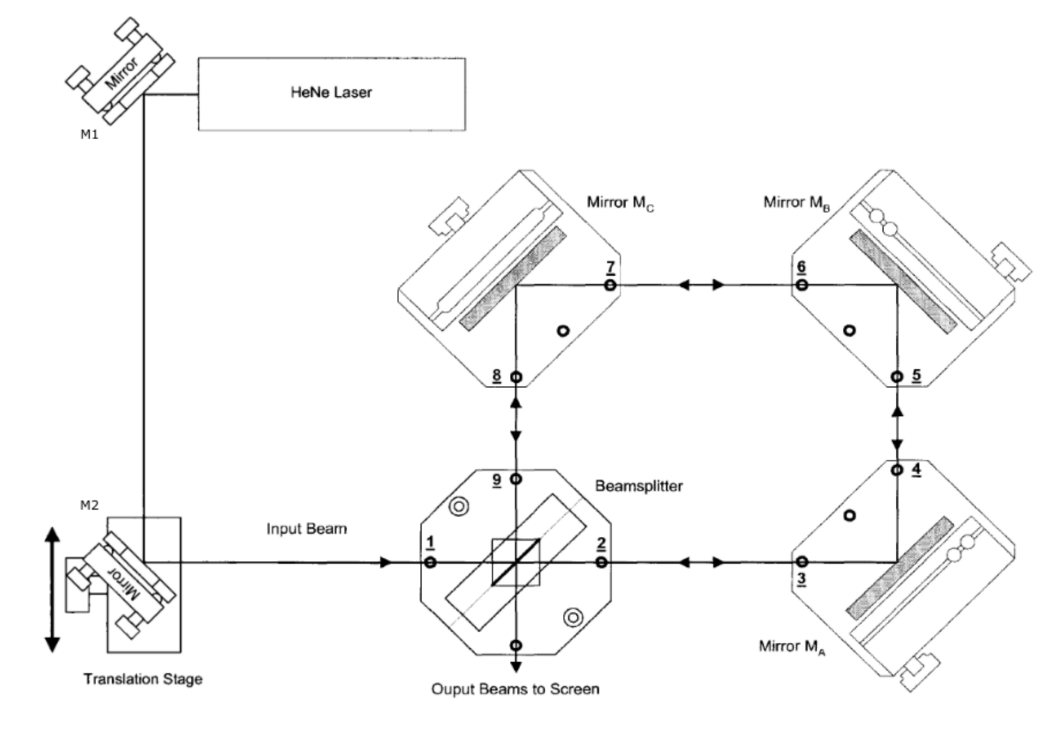
\includegraphics[width = 0.6\textwidth]{pictures/Sagnac.png}
          \caption{In der Abbildung ist der schematische Aufbau eine Sagnac-Interferometers dargestellt. Unser Aufbau beinhaltet zusätzlich einen weiteren Strahlteiler, der den Strahl 1:1 auf zwei Photdioden aufteilt, um die Messung per Differenzspannungsmethode zu ermöglichen. Entnommen aus \cite{tu_dortmund_versuchsanleitung_2021-3}}
          \label{fig:Aufbau}
        \end{figure}

        \FloatBarrier

        \noindent
        Der experimentelle Aufbau zur Bestimmung der Brechungsindezes besteht aus einem Sagnac-Interferometer~\ref{fig:Aufbau}, in das ein Laserstrahl der Wellenlänge \SI{632.990}{\nano\metre} eingespeist wird. 
        Der das Sagnac-Interferometer verlassende Strahl trifft auf einen \textit{polarizing beam splitter cube} (PBSC) und wird von diesem in seine vertikale und horizontale Polarisationskomponenten zerlegt.
        Dabei erhälteine der beiden Komponenten eine Phasenverschiebung von 180° relativ zur anderen Komponente, sodass die vorher in Phase schwingenden Komponenten nun gegenphasig schwingen. Daraufhin 
        werden die beiden Komponenten jeweils auf eine Photodiode geleitet. Die beiden Photdioden sind an ein Gerät gekoppelt, das die Differenz der Photodiodenspannungen misst. Diese Differenzspannung wird 
        auf einem Oszilloskop abgebildet. Aufgrund der gegenphasigen Schwingung der Kompoonenten sind die Maxima und Minima der Schwingung größer und die Nulldurchgänge daher stärker ausgeprägt. 


    \subsection{Justierung}
        Bevor mit den Messungen begonnen werden kann, muss das Sagnac-Interferometer justiert werden, sodass die zwei Strahlen parallel zueinander laufen. Dazu wird zunächst ein einzelner Strahl über zwei 
        Lochblenden justiert. Die Justierung erfolgt immer mit zwei Spiegeln, die jeweils zum justieren einer Lochblende genutzt werden. Das Justieren per Spiegel wird wiederholt, bis der Strahl an allen 
        Spiegeln des Interferometers genau die Lochblenden trifft. Nun wird der Strahl in zwei parallele Strahlen aufgespalten, welche durch die Vorjustierung bereits parallel laufen sollten. Für einen 
        perfekten Strahlengang wird mit nun vier Lochblenden eine Feinjustierung durchgeführt. \newline
        Bei korrekter Justierung sollten die beiden Strahlen nach Verlassen des Interferometers wieder genau parallel ineinander liegen und auf einem Schirm wäre nur ein Punkt zu sehen. Bei konstruktiver
        beziehungsweise destruktiver Interferenz müsste dieser Punkt entweder seine maximale Helligkeit erreichen oder komplett verschwinden. Wenn die Strahlen nicht genau übereinander liegen, ist ein 
        Interferenzmuster aus Strichen zu sehen. Um die Parallelität zu prüfen, werden Glasplättchen in den Strahlengang gehalten und rotiert, sodass die beiden Strahlen einen Phasenunterschied erhalten.
        Ihr Winkel zum Strahl wird gedreht und das Verhalten der interferierenden Strahle kann beobachtet werden. Nun wird wieder mit den Spiegeln im Interferometer fein justiert, bis das Interferenzverhalten
        dem zweier parallel ineinander liegenden Strahlen am nächsten kommt.

    \subsection{Kontrastbestimmung}
        Wenn diese Konfiguration erreicht ist, wird der Kontrast in Abhängigkeit von der Polarisation des einfallenden Lichtes gemessen. Dazu wird die Polarisation des Lichts, bevor es auf den Strahlteiler des
        Interferometers trifft, durch einen Polarisationsfilter festgelegt. Der Kontrast ergibt sich dann durch eine Intensitätsmessung der interferierenden Strahlen bei maximaler konstruktiver und maximaler
        destruktiver Interferenz. 

    \subsection{Messung des Brechungsindezes von Glas}
        Wieder werden zwei Glasplättchen, die bereits eine relative Verdrehung von $10\deg$ besitzen, in die parallel laufenden Strahlen gestellt. Die beiden Plättchen sind auf einem Zylinder befestigt und 
        werden um insgesamt $10\deg$ gedreht. Dabei wird die Anzahl der Interferenzminima  oder -maxima über die Differenzspannungsmethode bestimmt, die äußere Einflüsse reduziert, indem sie die Spannung 
        zweier Photodioden subtrahiert und jedem Maximum beziehungsweise Minimum einen Nulldurchgang zuordnet. Diese Messung wird insgesamt 10 mal wiederholt.

    \subsection{Messung des Brechungsindezes von Luft}
        Um den Brechungsindex von Luft zu ermitteln, wird wieder ein Gangunterschied zwischen den beiden Strahlen erzeugt. Dies wird erreicht, indem einer der Strahlen eine Gaszelle durchquert, während der 
        andere Strahl ungestört propagiert. Um die Phasendifferenz zu variieren wird der Druck in der Gaszelle zunächst auf 6 mbar gesenkt und anschlißend in 50 mbar-Schritten erhöht, bis wieder der Normaldruck
        des Raumes erreicht wird. Während des Prozesses wird wieder die Anzahl der Nulldurchgänge per Differenzspannungsmethode gemessen. Diese Messung wird 3 mal durchgeführt.
        
